\documentclass[11pt,reqno,final,pdftex]{amsart}\usepackage[]{graphicx}\usepackage[]{color}
%% maxwidth is the original width if it is less than linewidth
%% otherwise use linewidth (to make sure the graphics do not exceed the margin)
\makeatletter
\def\maxwidth{ %
  \ifdim\Gin@nat@width>\linewidth
    \linewidth
  \else
    \Gin@nat@width
  \fi
}
\makeatother

\definecolor{fgcolor}{rgb}{0.345, 0.345, 0.345}
\newcommand{\hlnum}[1]{\textcolor[rgb]{0.686,0.059,0.569}{#1}}%
\newcommand{\hlstr}[1]{\textcolor[rgb]{0.192,0.494,0.8}{#1}}%
\newcommand{\hlcom}[1]{\textcolor[rgb]{0.678,0.584,0.686}{\textit{#1}}}%
\newcommand{\hlopt}[1]{\textcolor[rgb]{0,0,0}{#1}}%
\newcommand{\hlstd}[1]{\textcolor[rgb]{0.345,0.345,0.345}{#1}}%
\newcommand{\hlkwa}[1]{\textcolor[rgb]{0.161,0.373,0.58}{\textbf{#1}}}%
\newcommand{\hlkwb}[1]{\textcolor[rgb]{0.69,0.353,0.396}{#1}}%
\newcommand{\hlkwc}[1]{\textcolor[rgb]{0.333,0.667,0.333}{#1}}%
\newcommand{\hlkwd}[1]{\textcolor[rgb]{0.737,0.353,0.396}{\textbf{#1}}}%

\usepackage{framed}
\makeatletter
\newenvironment{kframe}{%
 \def\at@end@of@kframe{}%
 \ifinner\ifhmode%
  \def\at@end@of@kframe{\end{minipage}}%
  \begin{minipage}{\columnwidth}%
 \fi\fi%
 \def\FrameCommand##1{\hskip\@totalleftmargin \hskip-\fboxsep
 \colorbox{shadecolor}{##1}\hskip-\fboxsep
     % There is no \\@totalrightmargin, so:
     \hskip-\linewidth \hskip-\@totalleftmargin \hskip\columnwidth}%
 \MakeFramed {\advance\hsize-\width
   \@totalleftmargin\z@ \linewidth\hsize
   \@setminipage}}%
 {\par\unskip\endMakeFramed%
 \at@end@of@kframe}
\makeatother

\definecolor{shadecolor}{rgb}{.97, .97, .97}
\definecolor{messagecolor}{rgb}{0, 0, 0}
\definecolor{warningcolor}{rgb}{1, 0, 1}
\definecolor{errorcolor}{rgb}{1, 0, 0}
\newenvironment{knitrout}{}{} % an empty environment to be redefined in TeX

\usepackage{alltt}
%% DO NOT DELETE OR CHANGE THE FOLLOWING TWO LINES!
%% $Revision$
%% $Date$
\usepackage[round,sort,elide]{natbib}
\usepackage{graphicx}
\usepackage{times}
\usepackage{rotating}
\usepackage{subfig}
\usepackage{color}
\newcommand{\aak}[1]{\textcolor{cyan}{#1}}
\newcommand{\mab}[1]{\textcolor{red}{#1}}
\newcommand{\cec}[1]{\textcolor{blue}{#1}}

\setlength{\textwidth}{6.25in}
\setlength{\textheight}{8.75in}
\setlength{\evensidemargin}{0in}
\setlength{\oddsidemargin}{0in}
\setlength{\topmargin}{-.35in}
\setlength{\parskip}{.1in}
\setlength{\parindent}{0in}

%% cleveref must be last loaded package
\usepackage[sort&compress]{cleveref}
\crefname{figure}{Fig.}{Figs.}
\Crefname{figure}{Fig.}{Figs.}
\crefname{table}{Table}{Tables}
\Crefname{table}{Tab.}{Tables}
\crefname{equation}{Eq.}{Eqs.}
\Crefname{equation}{Eq.}{Eqs.}
\crefname{appendix}{Appendix}{Appendices}
\Crefname{appendix}{Appendix}{Appendices}
\creflabelformat{equation}{#2#1#3}
\newcommand{\crefrangeconjunction}{--}
\newcommand{\creflastconjunction}{, and~}

\theoremstyle{plain}
\newtheorem{thm}{Theorem}
\newtheorem{corol}[thm]{Corollary}
\newtheorem{prop}[thm]{Proposition}
\newtheorem{lemma}[thm]{Lemma}
\newtheorem{defn}[thm]{Definition}
\newtheorem{hyp}[thm]{Hypothesis}
\newtheorem{example}[thm]{Example}
\newtheorem{conj}[thm]{Conjecture}
\newtheorem{algorithm}[thm]{Algorithm}
\newtheorem{remark}{Remark}
\renewcommand\thethm{\arabic{thm}}
\renewcommand{\theremark}{}

\numberwithin{equation}{part}
\renewcommand\theequation{\arabic{equation}}
\renewcommand\thesection{\arabic{section}}
\renewcommand\thesubsection{\thesection.\arabic{subsection}}
\renewcommand\thefigure{\arabic{figure}}
\renewcommand\thetable{\arabic{table}}
\renewcommand\thefootnote{\arabic{footnote}}

\newcommand\scinot[2]{$#1 \times 10^{#2}$}
\newcommand{\code}[1]{\texttt{#1}}
\newcommand{\pkg}[1]{\textsf{#1}}
\newcommand{\dlta}[1]{{\Delta}{#1}}
\newcommand{\Prob}[1]{\mathbb{P}\left[#1\right]}
\newcommand{\Expect}[1]{\mathbb{E}\left[#1\right]}
\newcommand{\Var}[1]{\mathrm{Var}\left[#1\right]}
\newcommand{\dd}[1]{\mathrm{d}{#1}}
\newcommand{\citetpos}[1]{\citeauthor{#1}'s \citeyearpar{#1}}
\IfFileExists{upquote.sty}{\usepackage{upquote}}{}
\begin{document}



\begin{figure}
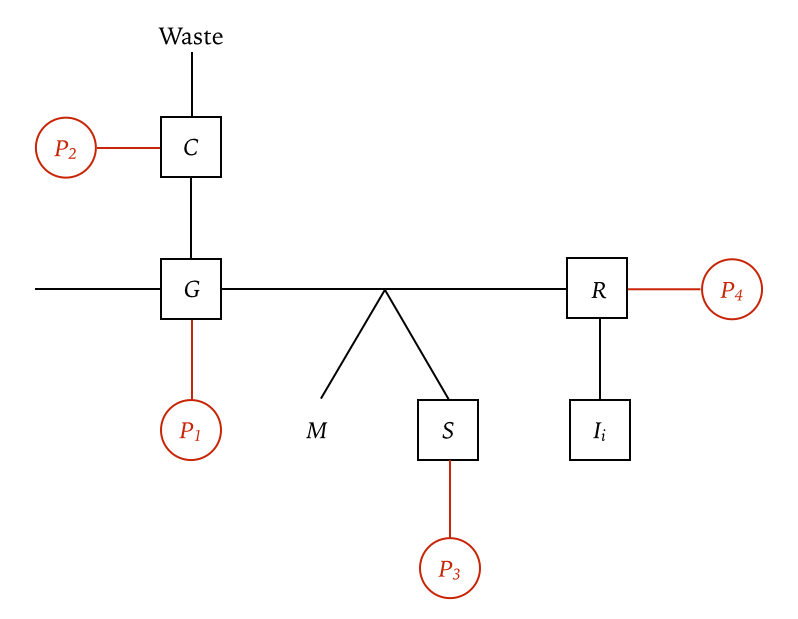
\includegraphics[width=\textwidth]{Macroparasite_DEB.png}
\caption{The basic model structure showing the state variables for the host (in boxes) and parasite (in circles). See the text for full details.}
\label{fig:model}
\end{figure}

The basic model (shown in Fig. \ref{fig:model}) defines three individual host state variables: $S(t)$, the structural biomass; $R(t)$, the reserve biomass; and $I_i(t)$, the biomass of the induced immune system.
We also need to consider the biomass of the constitutive immune system, $I_c(t)$, but as we discuss below, this has a very simple dependence on the other state variables.
There is also one state variable for the parasite biomass, $P(t)$.

Note that $I_c(t)$ is the total biomass of all of the immune cells present in a host prior to parasite invasion, regardless of whether these cells are part of the innate immune system (e.g., eosinophils, macrophages) or the adaptive immune system (e.g., lymphocytes).
Similarly, $I_i(t)$ is the total biomass of all the immune cells produced in response to parasite invasion, regardless of their specific type.

We make the assumption that we are modeling the biology of animals with determinant growth, so we move away from the standard DEB model assumptions.
In particular, we make some very strong assumptions about the growth of structural biomass and constitutive immune biomass.

\subsection*{Model assumptions:}
\begin{itemize}
\item individuals have a genetically predetermined growth pattern in structural biomass that is independent of how much they are eating;
\item individuals have a genetically predetermined constitutive immune system that depends only on the total weight $(S(t)+R(t))$ of the organism, not on how much they are eating;
\item total maintenance costs depend on the total weight and the biomasses of the constitutive and induced immune systems;
\item all assimilated biomass that is not used for maintenance or structural growth is stored in reserves;
\item the induced immune response ``paid'' using reserve biomass.
\end{itemize}

\subsection*{Reserve dynamics}
The key equation for host dynamics is the equation for reserve dynamics, which is
\begin{equation}
\frac{dR}{dt}=\epsilon _R\left[\epsilon _A I-M-C_G\right]-b R P,
\end{equation}
where:
\begin{itemize}
\item $A$ is the ingestion rate (which depends on the abundance of food, as well as on both $S(t)$ and $R(t)$, and may depend on $P(t)$ for parasites that manipulate host foraging behavior);
\item $\epsilon _A$ is assimilation efficiency (which may depend on the abundance of food and $R(t)$ for hosts that increase assimilation efficiency when food is scarce or condition is poor, and may depend on $P(t)$ for parasites that manipulate the amount of ingesta going to waste, like whipworms);
\item $M$ is the total maintenance rate;
\item $C_G$ is the cost of growth in structural biomass;
\item $\epsilon _R$ is the cost of converting assimilated resource into reserve biomass;
\item $bRP$ is the allocation of reserve to fuel an induced immune response. Note that this makes the induced response independent of the number of induced (or constitutive) immune cells. This kind of model has been studied by other authors \citep{Bonhoeffer1994,Alizon2005,Fenton2006,Hamilton2008}, and reflects the fact that the immune-parasite interaction is not really a predator-prey interaction in the sense that the immune response is not stimulated by direction contact between immune cells and parasites.
\end{itemize}

\subsection*{Ingestion}
It has been suggested that ingestion scales with surface area, so that ingestion should depend on $(S(t)+R(t))^{2/3}$. Since we are considering
ad lib feeding right now, we can ignore any potential nonlinearities in feeding, as food abundance is always saturating.
In this case,
\begin{equation}
I=I_{\max }(S+R){}^{2/3},
\end{equation}
where:
\begin{itemize}
\item $I_{\max }$ is the maximum surface-area-specific ingestion rate.
\end{itemize}

\subsection*{Maintenance}
An organism must pay the metabolic cost of all of its cells, which means that a model of maintenance might be
\begin{equation}
M=m(S+R)+m_cI_c+m_iI_i,
\end{equation}
where:
\begin{itemize}
\item $m$ is the maintenance rate for weight, which is assumed to be the same for structure and reserves;
\item $m_c$ is the maintenance rate for constitutive immune biomass;
\item $m_i$ is the maintenance rate for induced immune biomass.
\end{itemize}


It may be reasonable to question whether there should be separate maintenance rates for structure $S(t)$ versus reserves $R(t)$, but this is
probably reasonable for the moment. I discuss the separate maintenance costs for constitutive versus induced immune biomass below.

\subsection*{Constitutive immune defense}
Rather than considering a dynamic constitutive immune defense, we instead assume that organisms maintain a constitutive immune biomass that is proportional to total biomass. To some extent, this makes biological sense: hosts should want to maintain a relatively constant level of surveillance, regardless of how much tissue they have. Therefore, we assume that the total biomass of constitutive defense is:
\begin{equation}
I_c=k(S+R),
\end{equation}
where:
\begin{itemize}
\item $k$ is the biomass of the constitutive immune system relative to the total biomass in weight ($k<<1$).
\end{itemize}


Note that we do not consider the cost of building these cells, or, more precisely, we assume that the building cost and the maintenance cost are identical. This is quite different from our assumptions for the induced immune response (discussed below).

\subsection*{ Induced immune response}
The derivation of the reserve dynamics equation implies a model for the induced immune response of
\begin{equation}
\frac{dI_i}{dt}=\epsilon _ib R P-\mu _II_i,
\end{equation}
where:
\begin{itemize}
\item $\epsilon _i$ is the cost of converting reserve biomass into \textit{ effective }induced immune biomass (see below);
\item $b$ is the rate reserve biomass is allocated to the immune system per unit of parasite biomass;
\item $\mu _I$ is the background rate that immune cells are lost.
\end{itemize}

With this model formulation, if an infection is cleared, the induced immune response returns to 0; we may, at some point in the future, want to consider the fact that some of the cells of the induced immune response become part of the constitutive immune system after infection (e.g., memory cells).

We can also make some assumptions about parameter values.
The induced immune response is very costly to develop because it is wasteful: lymphocytes go through a process of differentiation followed by somatic selection that culls most of these newly produced cells.
Maintaining the effective cells should be comparatively cheap.
Most likely, what this would imply is that the parameter $b$ should be relatively large - lots of energy is invested in the induced immune response - but $\epsilon _I$ should be relatively small - most of that energy is spent building immune cells that will not actually be effective.
On the other hand, the cost of maintaining the effective induced immune cells $m_i$ should be different from either $b$ or $\epsilon_i$, different from the case of constitutive immune biomass.

\subsection*{Cost of growth}
This one turns out be slightly more complicated.
Let's start with the equation for structural biomass.

If you assume that structural biomass $S$ scales with structural length $L$ as $S =\epsilon L^3$, and you assume that structural length
follows a von Bertalanffy equation, then
\begin{align}
\frac{dS}{dt} &=\frac{d\left(\epsilon  L^3\right)}{\text{dt}} \\
& =3\epsilon  L^2 \frac{dL}{dt} \\
& =3 \epsilon  L^2 \left(\gamma \left(L_{\infty}-L\right)\right) \\
& =3 \gamma \left(\epsilon  L^2 L_{\infty}-\epsilon  L^3\right) \\
& =3 \gamma \left(\epsilon  L^2L_{\infty }-S\right).
\end{align}

Note that $S^{2/3}=\epsilon ^{2/3}L^2$, or $L^2=S^{2/3}/\epsilon ^{2/3}$, so
\begin{equation}
\frac{dS}{dt}=3\gamma  \left(\epsilon ^{1/3}L_{\infty }S^{2/3}-S\right).
\end{equation}
If a unit of structural biomass increase costs $\epsilon _G$, then the total cost for structural growth is
\begin{equation}
C_G = \epsilon _G 3\gamma  \left(\epsilon ^{1/3}L_{\infty }S^{2/3}-S\right).
\end{equation}
This agrees with Anieke's derivation.
Most of these parameters have probably already been estimated (for mice, anyway; see the back of Kooijman's book), including the shape parameter $\epsilon$, the maximum structural length $L_{\infty }$, and the growth rate in structure $\gamma$.

Of course, it is possible to directly solve the von Bertalanffy growth equation, so we could eliminate one equation from the model by simply solving for the size of the animal at any age.
In particular, $\frac{dL}{dt}=\gamma \left(L_{\infty }-L\right), \text{with} L(0)=L_b$, has the solution $L(t)=L_{\infty }+\left(L_b-L_{\infty}\right)e^{-\gamma t}$, and the structural biomass $S(t)=\epsilon  L(t)^3$.

However, if the parasite utilizes structure as a resource, the structural growth equation has to be modified to include parasitism, and we will no longer be able to solve the equation.
In particular, the structural biomass equation will become
\begin{equation}
\frac{dS}{dt}=3\gamma  \left(\epsilon ^{1/3}L_{\infty }S^{2/3}-S\right)-\frac{k S P}{h+S}.
\end{equation}
However, we can still make use of the analytical solution: when the parasite is using up structural biomass as resource, the amount allocated to growth (i.e., $C_G$)should increase in proportion to how far the host is from it's target structural biomass.
That is, define
\begin{equation}
S_{\text{target}}(t)=\epsilon \left(\left(L_b-L_{\infty }\right) e^{-\gamma  t}+L_{\infty }\right)^3,
\end{equation} and let the solution of the differential equation for $\frac{dS}{dt}$ give the actual weight.

It seems to make sense to me, at this point, to imagine that what happens when an organism is below its target structural biomass is to increase the amount of energy allocated to growth to attempt to accelerate the growth rate (e.g., ``catch-up'' growth).
That is, the parameter $\gamma$ should become a function of the difference between the target structural biomass and the actual structural biomass.
For example, if you let
\begin{equation}
\gamma =\gamma _{\min }+\gamma _{\text{catchup}}\left(\frac{S_{\text{target}}(t)}{S(t)}-1\right),
\end{equation}
then whenever $S(t)<S_{\text{target}}(t)$, then $\gamma$ increases, increasing the allocation of energy towards growth and enabling the \textit{possibility} of catch-up growth.
Of course, if there is a parasite that is also sucking up biomass, the host may or may not actually be able to catch up.
If the parasite is cleared, the host will have an increased growth rate until $S(t)=S_{\text{target}}(t)$, and then the growth rate will fall back to normal.

Thus, we have equations for the rate of structural biomass increase, the growth rate, and cost of growth:
\begin{align}
\frac{dS}{dt} &= 3\gamma  \left(\epsilon ^{1/3}L_{\infty }S(t)^{2/3}-S(t)\right)-\frac{k S(t) P(t)}{h+S(t)} \\
C_G(t)&=\epsilon _G 3\gamma  \left(\epsilon ^{1/3}L_{\infty }S(t)^{2/3}-S(t)\right) \\
\gamma &=\gamma _{\min }+\gamma _{\text{catchup}}\left(\frac{S_{\text{target}}(t)}{S(t)}-1\right) \\
S_{\text{target}}(t) &=\epsilon  \left(\left(L_b-L_{\infty }\right) e^{-\gamma  t}+L_{\infty }\right)^3
\end{align}
For non-parasitized hosts, or hosts parasitized by parasites targeting other sources of biomass, then $S(t)=S_{\text{target}}(t)$, and you only need two of the above equations.

\section*{Model equations, including parasitism}
As seen in Fig. \ref{fig:model}, we consider 4 kinds of parasite: $P_1$ are parasites of ingestion; $P_2$ are parasites of waste; $P_3$ are parasites of structure; and $P_4$ are parasites of reserves.
One of the main differences between these parasites, from a modeling perspective, that we need to deal with is that $P_1$ and $P_2$ are parasitizing a \emph{flow} of biomass, whereas $P_3$ and $P_4$ are parasitizing \emph{stored} biomass.
This makes the models different for each.
For example, it makes sense to imagine that $P_{1,2}$ capture some \emph{proportion} of the flow, whereas $P_{3,4}$ have a functional response.
In particular, for $P_1$ and $P_2$:
\begin{align}
\frac{dP_1}{dt} &= \epsilon_P \sigma P_1 I - \mu_P P_1 - \mu_c P_1 I_c - \mu_i P_1 I_i,\\
\frac{dP_2}{dt} &= \epsilon_P \sigma P_2 (1-\epsilon_A) I - \mu_P P_2  \mu_c P_2 I_c - \mu_i P_2 I_i,
\end{align}
where $\sigma P_1$ is the fraction of the flow captured by the parasite, $\epsilon_P$ is the cost of converting between biomasses, $\mu_P$ is the background rate of biomass loss, and $\mu_{c,i}$ are the loss rates due to the constitutive and induced immune responses, respectively.

For $P_3$ and $P_4$:
\begin{align}
\frac{dP_3}{dt} &= \epsilon_P \frac{k_S S P}{h_S + S} - \mu_P P_3 - \mu_c P_3 I_c - \mu_i P_3 I_i,\\
\frac{dP_4}{dt} &= \epsilon_P \frac{k_R R P}{h_R + R} - \mu_P P_4 - \mu_c P_4 I_c - \mu_i P_4 I_i,
\end{align}
where $k_{S,R}$ is the parasite's ``attack rate'' and $h_{S,R}$ is a half-saturation constant for the parasite.

I dislike that $P_{1,2}$ and $P_{3,4}$ have very different per-capita growth rate expressions.

\bibliographystyle{ecology.bst}
\bibliography{Biblio.bib}

\end{document}
